\documentclass[11pt,a4]{jarticle}
\usepackage[top=25truemm,bottom=30truemm,left=20truemm,right=20truemm]{geometry}
\usepackage{graphicx}
\usepackage{comment}
\begin{document}

\title{ねじり振動系}
\author{レポート提出者: 平松信義、共同実験者: 森本颯太}
\date{実験日: 平成29年6月12日、13日\\レポート提出日: 平成29年6月20日}
\maketitle
\tableofcontents

\section{実験の目的}
光に対する物質の振る舞いや電気回路、耐震設計など、振動現象はさまざまな分野に現れ、普遍的かつ重要である。本実験では機械的なねじり振動系の振る舞いを調べ、振動現象に一般に現れる性質の理解を目的とする。

\section{実験方法}
本実験ではねじり機械振動系を用いた。
図\ref{fig:schematics}に実験装置の構成の模式図を示す。
ピアノ線に吊るされた円盤に単振動するトルクを直流モータから与え、振動状態を励起した。変位はロータリエンコーダとフォトカプラで検出し、DA変換をした後オシロスコープで読み取った。
円盤と連結したダンピングシリンダをシリコンオイルに挿入し、その挿入する深さ(液浸部の深さ)を変化させることで粘性要の強さを制御した。
\begin{figure}[htbp]
   \begin{center}
    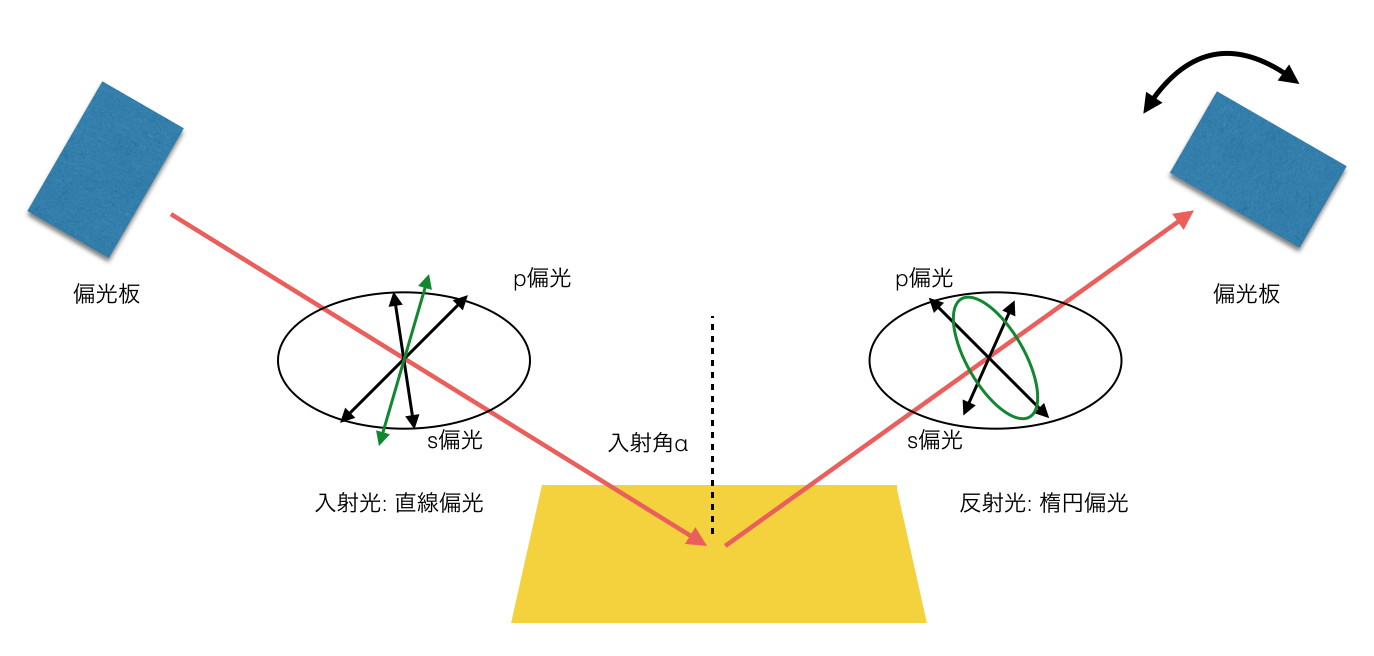
\includegraphics[width=0.6\hsize]{./schematics.eps}
    \caption{実験装置の模式図}
     \label{fig:schematics}
   \end{center}
\end{figure}


ねじり振動系は十分にねじれの振幅が小さければ、以下の微分方程式(Voigt model)でモデル化できる。
\begin{equation}
A \frac{d^2 x}{dt^2} + B \frac{dx}{dt} + C x =  D cos \omega t  
\label{eq:Voigt_model}
\end{equation}
ここでAは慣性モーメント、Bは粘性抵抗係数、Cはねじり弾性モーメント、Dは駆動トルクの振幅である。駆動トルクを入力しないときD=0であり、粘性要素を無視したときB=0である。

\subsection{固有振動数の測定}
ダンピングシリンダをシリコンオイルから抜いた状態で実験を行う。
駆動トルクにより有限の振幅を系に与えたあと駆動トルクを切ると、系は一定の振幅で自由振動する。このときの振動数を測定した。

\subsection{強制振動}
ダンピングシリンダをシリコンオイル内に挿入し、その深さを95mmで固定した。
その状態で駆動トルクを系に与えて、強制振動状態を引き起こす。ねじれの変位振幅と、駆動トルクに対する変位の位相差を調べた。

\subsection{減衰振動}
ダンピングシリンダの液浸部の深さZを変えて、粘性抵抗係数Bを変化させる。
このとき減衰振動の振幅が1周期あたりどれだけ減衰するか調べた。

\section{実験結果}
\subsection{固有振動数の測定}
オシロスコープから振動の数周期分の時間を読み取って振動数を計算し、さらにそれを繰り返し測定して平均した。固有振動数fは$0.910 \pm 0.01$Hzと見積もれた。

\subsection{強制振動}
駆動トルクの周波数を変えながら系に入力して、系の変位の振幅と、駆動トルクに対する変位の位相遅れを測定した。ここでトルクの周波数を徐々に大きくしてゆく条件(登り/ascending)と、徐々に小さくしてゆく条件(下り/descending)の二通りで実験を行った。
入力したトルクの周波数に対する角度の振幅を図\ref{fig:Lorenz}にプロットし、データをLorenz関数にフィッテイングしたものを同図上に曲線で示した。その中心周波数$f_c$と半値全幅$FWHM$、Q値を表\ref{tab:Q_value_etc}に示した。ここで半値全幅は振幅の二乗に比例するエネルギーの領域で計算した。またQ値は以下で与えられる。
\begin{equation}
Q =  \frac{f_c}{FWHM}
\label{eq:Q1}
\end{equation}

図\ref{fig:phase}に周波数に対する位相をプロットした。中心周波数$f_c$の近くで位相が90度ずれており、それより周波数が小さいと位相遅れは0度に近づき、大きいと位相遅れは180度に近づいてゆくことが分かる。

\begin{figure}[htbp]
 \begin{minipage}{0.5\hsize}
   \begin{center}
    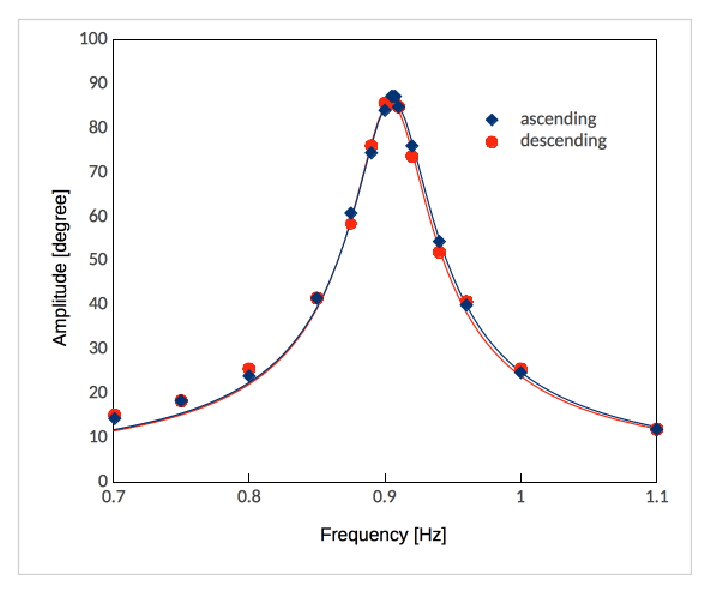
\includegraphics[width=0.8\hsize]{./Lorenz.eps}
    \caption{振幅の周波数依存性}
     \label{fig:Lorenz}
   \end{center}
 \end{minipage}
 \begin{minipage}{0.5\hsize}
   \begin{center}
    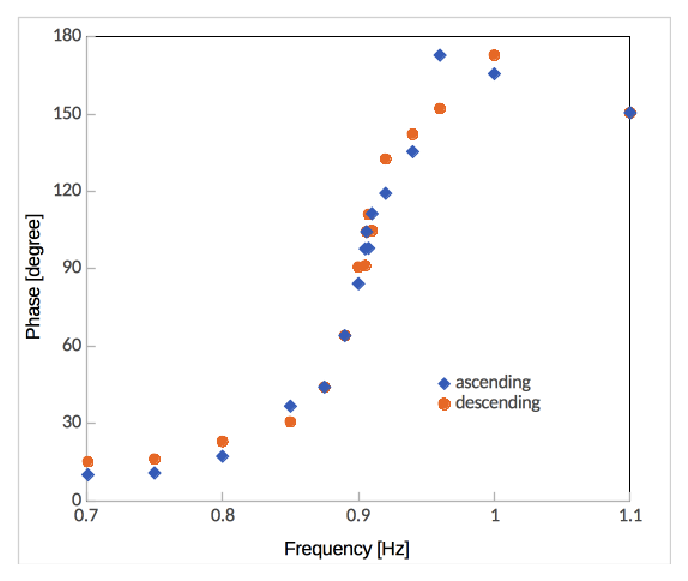
\includegraphics[width=0.8\hsize]{./phase.eps}
    \caption{位相の周波数依存性}
     \label{fig:phase}
   \end{center}
 \end{minipage}
\end{figure}

\begin{table}[htbp]
   \begin{center}
  \begin{tabular}{c|ccc}
    & 中心周波数  & 半値全幅 & Q値\\ \hline
    登り& 0.905 Hz & 0.0569 Hz & 15.9\\
    下り& 0.904 Hz & 0.0556 Hz & 16.3
  \end{tabular}
  \label{tab:Q_value_etc}
     \end{center}
       \caption{中心周波数と半値全幅、Q値}
\end{table}

以降トルクの周波数を徐々に大きくしてゆく条件を考える。
強制振動の定常状態において、外力とねじれ変位の複素振幅比を複素感受率$\chi$、外力と角速度の複素振幅比を複素移動度$\mu$とする。図\ref{fig:Lorenz}、\ref{fig:phase}に示した振幅Aと位相$\phi$から、$\chi \propto Aexp(i\phi)$と$\mu \propto A i\omega exp(i\phi)$を以下で計算し、それらの周波数依存性を図\ref{fig:chi_frequency}、\ref{fig:mu_frequency}にプロットした。中心周波数付近で$\chi$の実部と$\mu$の虚部は極値をとる。また中心周波数付近で$\chi$の虚部と$\mu$の実部は値0をとる。
また$\mu$について複素平面上にプロットしたものを図\ref{fig:mu}に示す。$\mu$はある正の実数を中心として原点付近を通る円を描いていることが見て取れる。
ただし$\chi$と$\mu$をプロットした図\ref{fig:chi_frequency}、\ref{fig:mu_frequency}、\ref{fig:mu}について、それぞれの単位は不定とした。

\begin{figure}[htbp]
 \begin{minipage}{0.5\hsize}
   \begin{center}
    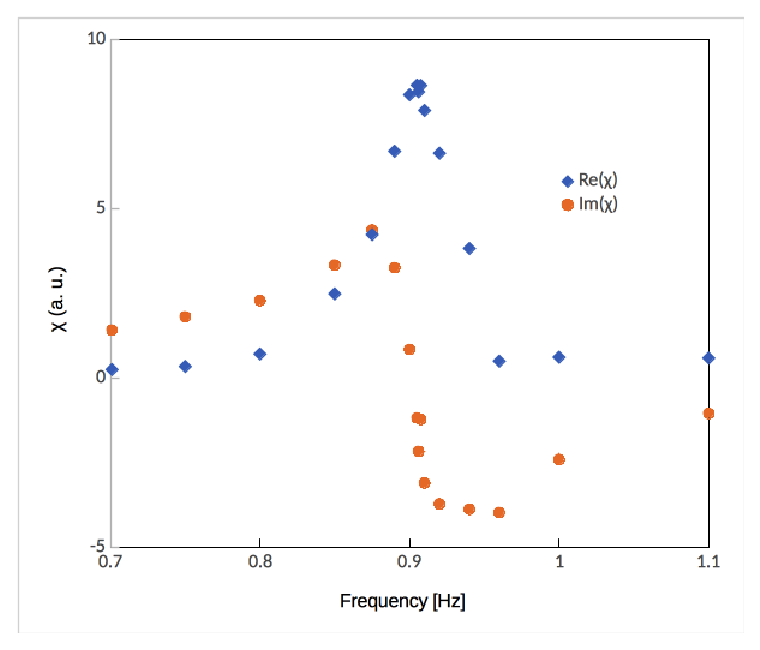
\includegraphics[width=0.9\hsize]{./chi_frequency.eps}
    \caption{$\chi$の周波数依存性}
     \label{fig:chi_frequency}
   \end{center}
 \end{minipage}
 \begin{minipage}{0.5\hsize}
   \begin{center}
    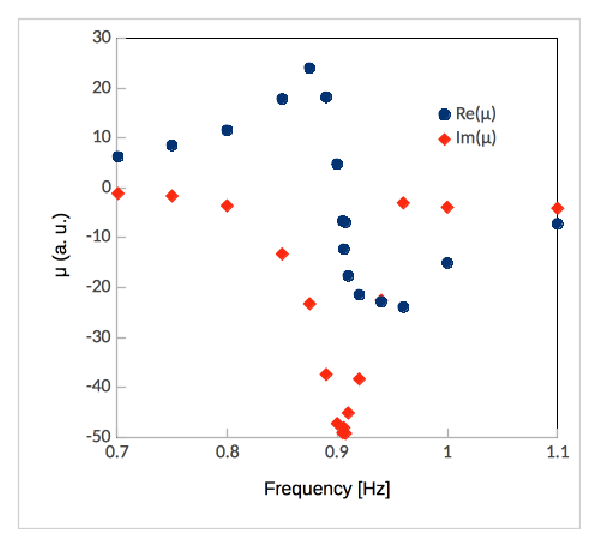
\includegraphics[width=0.9\hsize]{./mu_frequency.eps}
    \caption{$\mu$の周波数依存性}
     \label{fig:mu_frequency}
   \end{center}
 \end{minipage}
\end{figure}

\begin{figure}[htbp]
   \begin{center}
    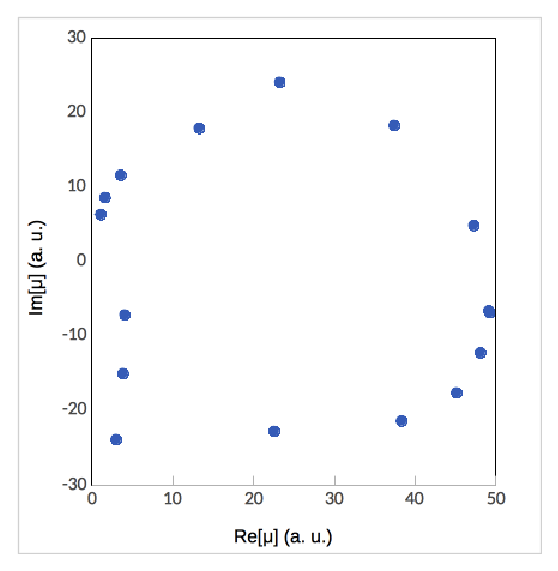
\includegraphics[width=0.4\hsize]{./mu.eps}
    \caption{強制振動}
     \label{fig:mu}
   \end{center}
\end{figure}

\subsection{減衰振動}
まずある液浸部の深さZで振幅を数周期ごとに記録し、最小二乗法を用いて一周期あたりの対数減衰率$\Lambda$を求めた。求めた対数減衰率$\Lambda$と粘性抵抗係数Bは式\ref{eq:B}の関係にある。
\begin{equation}
B =  2A f \Lambda
\label{eq:B}
\end{equation}
ここでfは固有振動数である。

同様の手続きを液浸部の深さZを変えながら行い、ZとBの関係を図\ref{fig:B}にプロットした。この図は青色の点で測定点を表し、青色の破線でその測定点の線形回帰直線を表す。またオレンジ色の実線はシリコンオイルの粘性率$\eta$を用いて、以下の式で計算した値である。
\begin{equation}
B =  4\pi \eta Z (r_2^{-2} -r_3^{-2} )^{-1}
\label{eq:B}
\end{equation}
ここで$r_2$はダンピングシリンダの半径、$r_3$はシリコンオイルを充填した油層の内径である。

実験値(青)の線形回帰直線の傾きは$1.22\times10^{-9} [kg\cdot m \cdot s]$で、計算値の傾きは$1.18\times10^{-9} [kg\cdot m \cdot s]$だった。

\begin{figure}[htbp]
   \begin{center}
    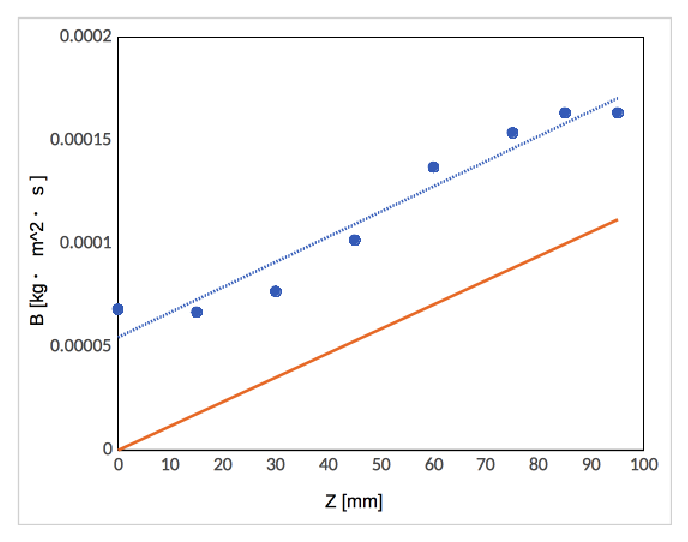
\includegraphics[width=0.6\hsize]{./B.eps}
    \caption{粘性抵抗係数Bと液浸部の深さZの関係}
     \label{fig:B}
   \end{center}
\end{figure}


\section{考察}
\subsection{固有振動数の測定}
十分に粘性が小さく、$B^2<<4AC$と仮定する。このとき慣性モーメントAとねじり弾性モーメントCを用いて、以下の式\ref{eq:estimation_beta}から固有周波数fが見積もれる。
\begin{equation}
f =  \frac{1}{2\pi}\sqrt{\frac{C}{A}-\frac{B^2}{4A^2}} \sim \frac{1}{2\pi}\sqrt{\frac{C}{A}}
\label{eq:estimation_beta}
\end{equation}
これから$f = 0.91 $Hz が計算できた。この計算で見積もった値と測定値$0.910 \pm 0.01$Hzは、計算値の有効桁数の範囲内で一致した。

\subsection{強制振動}
図\ref{fig:Lorenz}で非線形フィッティングしたローレンツ型関数とデータは良く一致している。これは式\ref{eq:Voigt_model}でモデル化できる強制振動現象に共通の特徴である。

固有振動数$f=0.910 \pm 0.01$Hzと強制振動スペクトルの中心周波数$fc=0.0905$Hz(または$0.904$Hz)はおおむね一致しているが、僅かに$f>f_c$である。これは強制振動では$B>0$であることと式\ref{eq:estimation_beta}から理解できる。

複素移動度$\mu$は慣性モーメントAと粘性抵抗係数B、ねじり弾性モーメントCを用いて以下のように表せる。
\begin{equation}
\mu = ( Ai \omega + B + \frac{C}{i \omega} ) ^{-1} 
\label{eq:mu}
\end{equation}

この表式の両辺から1/2Bを引くと、次が得られる。
\begin{equation}
|\mu - \frac{1}{2B}| = | \frac{ - Ai \omega + B - C/i \omega}{ Ai \omega + B + C/i \omega}| \frac{1}{2B} = \frac{1}{2B} 
\label{eq:circle}
\end{equation}
これから図\ref{fig:mu}で$\mu$が、ある正の実数を中心として原点付近を通る円を描くことの背景が理解できる。

\subsection{減衰振動}
実験値(青)の線形回帰直線の傾き$1.22\times10^{-9} [kg\cdot m \cdot s]$と計算値の傾き$1.18\times10^{-9} [kg\cdot m \cdot s]$は、良い精度で一致している。しかし、どのZの値でもBの実験値はBの計算値に対して一定の差(オフセット)の分だけ大きい。このオフセットはシリンダ底面での粘性抵抗やモータの抵抗など、計算モデルに算入していない効果によると筆者は考える。

対数減衰率$\Lambda$とQ値は、以下のように反比例の関係にあることが知られている。
\begin{equation}
Q =  \frac{\pi}{\Lambda}
\label{eq:B}
\end{equation}
これからZ=95mmの条件でQ値は22.9だった。強制振動スペクトルから求めたQ値の15.9と16.3(表\ref{tab:Q_value_etc}に示した)とおおむね一致している。

実験に用いた条件で$B^2 < 2.27\times10^{-8} [kg^2 \cdot m^4 \cdot s^2] $が分かった。
実験系の慣性モーメントAとねじり弾性モーメントCから、$4AC= 5.58\times10^{-5} [kg^2 \cdot m^4 \cdot s^2]$ である。したがって$B^2<<4AC$が示せた。

\section{結論}
自由振動から計算した固有周波数$f$と強制振動スペクトルの中心周波数$f_c$はおおむね一致した。
強制振動の振幅スペクトルはローレンツ型関数で精度よく近似できた。したがって本実験で用いた系はVoigt modelで精度よくモデル化できていることを確認した。
また液浸部の深さZと粘性抵抗係数Bは、高い精度で線形関係にあることを示した。


\end{document}